\documentclass[a4paper,12pt]{article}
\usepackage[utf8]{inputenc}
\usepackage[T1]{fontenc}
\usepackage[hungarian]{babel}
\usepackage{graphicx}
\usepackage{geometry}
\geometry{a4paper,
		     tmargin = 35mm, 
		     lmargin = 25mm,
		     rmargin = 30mm,
		     bmargin = 30mm}
\usepackage{mathtools}
\usepackage{amsmath}
\usepackage{color}
\usepackage{setspace}
\usepackage{amsmath,amssymb}
\usepackage{float}
\usepackage{hyperref}

\usepackage{indentfirst}
\usepackage{subfig}

\usepackage{siunitx}

\renewcommand\thesection{\Roman{section}}

\begin{document}

\linespread{1.25}

\begin{titlepage}

	\centering
	
\includegraphics[width=0.66\textwidth]{elte.jpg}\par\vspace{1cm}
	{\scshape\LARGE ELTE TTK \par}
	\vspace{3cm}
	{\scshape\Large Elektronmikroszkópia \par}
	\vspace{1cm}
	{\large\itshape Olar Alex\par}
	\vspace{3cm}
	{\large 2018 \par}
	
\end{titlepage}

\tableofcontents

\newpage

\section{Elméleti összefoglaló, mérési eszközök}

\vspace{5mm}

\par A mérés során egy transzmissziós elektronmikroszkópot használtunk, mellyel különböző mintákat vizsgáltunk meg. A feladatunk a mikroszkóp kameraállandójának meghatározása volt, majd ezután egy $Si$ mintán végeztük diffrakciós mérést.

\vspace{5mm}

\par A mérés során a képeket 'image plate'-re rögzítettük, amiket előhívás után, elektronikus formában megkaptunk.

\section{Kalibráció}

\vspace{5mm}

\par Polikristályos nikkelt használva a klaibráláshoz igen egyszerű összefüggést kapunk köbös rácsra

\vspace{5mm}

\begin{equation}
R_{hkl} = \frac{L\lambda}{a}\sqrt{h^{2} + k^{2} + l^{2}}
\end{equation}

\vspace{5mm}

\par Ahol $a$ a rácsállandó, $\lambda$ az elektron hullámhossz. Természetesen ez még ennél is egyszerűbb hiszen $d = \frac{a}{\sqrt{h^{2} + k^{2} + l^{2}}}$, ami meg van adva a \url{http://www.energia.mta.hu/~labar/Ni_cF4_04-010-6148.pdf} alatt.

\vspace{5mm}

\begin{figure}[!htb]
\centering
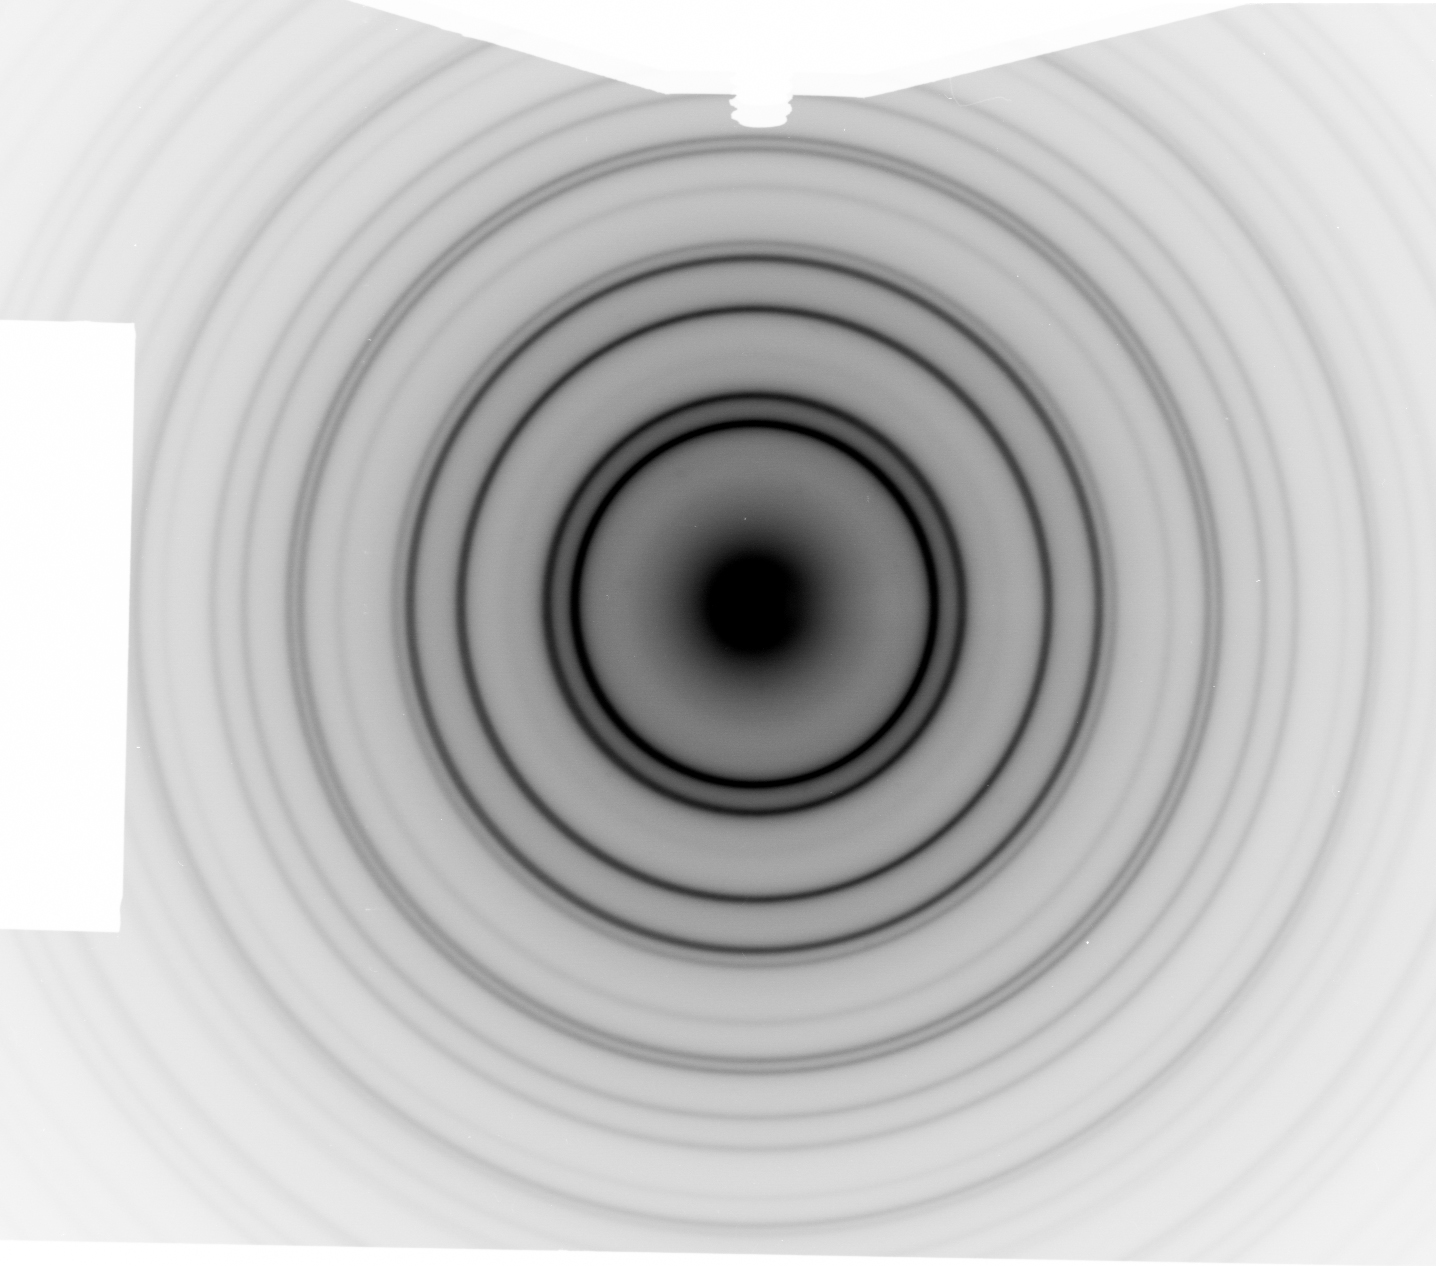
\includegraphics[width=0.55\linewidth]{./Ni-Calibration.jpg}
\caption{ A nikkel gyűrűs diffrakciós képe, ami a polikristályos elrendeződés miatt alakul ki. A kalibrációhoz függőlegesen a 754. pixelnél vettem ki egy oszlopot}
\end{figure}

\vspace{5mm}

\par A kalibrációhoz használt intenzitás csúcsokat ábrázolva

\vspace{5mm}

\begin{figure}[!htb]
\centering
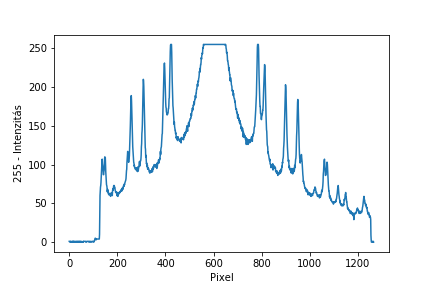
\includegraphics[width=0.65\linewidth]{./kalib.png}
\caption{ Az intenzitás (255 - intenzitásként) van ábrázolva, hogy a fekete gyűrűk legyenek a csúcsok}
\end{figure}

\vspace{5mm}

\par A csúcsokra Gauss-függvényeket illesztettem konstans háttérrel. A középső foltra nem illesztettem, csak az azt határoló 8 csúcsra. Ebből kaptam 4 csúcsot, melyek rendre

\vspace{5mm}

\begin{center}
\begin{tabular}{|c|c|}
\hline
Csúcs helye [$pixel$] & $\Delta$ csúcs helye [$pixel$] \\
\hline
257.74 & 0.11 \\
\hline
308.49 & 0.01 \\
\hline
395.56 & 0.05 \\
\hline
422.93 & 0.11 \\
\hline
784.17 & 0.07 \\
\hline
812.01 & 0.09 \\
\hline
899.2 & 0.07 \\
\hline
950.06 & 0.05 \\
\hline
\end{tabular}
\end{center}

\vspace{5mm}

\par Ebből már könnyen számolhatóak a sugarak, mert csak páronként ki kell vonni egymásból a mért értékeket (első négyből a második négyet). A hibát négyzetes hibaterjedéssel számoltam.

\vspace{5mm}

\par Sorrendben ezek a gyűrűk sugarai, a legintenzívebb pontot kihagyva. Az ezekhez tartozó $d$ távolságokat a korábbi linkről véve:

\vspace{5mm}

\begin{center}
\begin{tabular}{|c|c|c|}
\hline
R [$pixel$] & $\Delta$R [$pixel$] & d [\si{\angstrom}] \\
\hline
180.62 & 0.13 & 2.037180\\
\hline
208.23 & 0.10 & 1.764250 \\
\hline
295.36 & 0.07 & 1.247510\\
\hline
346.16 & 0.12 & 1.063880\\
\hline
\end{tabular}
\end{center}

\vspace{5mm}

\par Egyenest illesztve tehát kapjuk a meredekségből a kameraállandót

\vspace{5mm}

\begin{figure}[!htb]
\centering
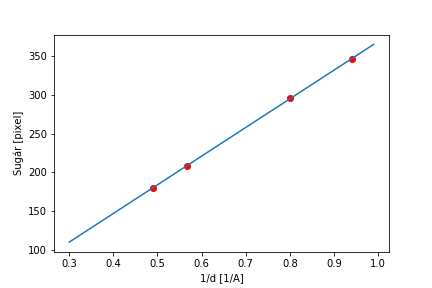
\includegraphics[width=0.45\linewidth]{./kalib_egyenes.png}
\caption{ Az intenzitás (255 - intenzitásként) van ábrázolva, hogy a fekete gyűrűk legyenek a csúcsok}
\end{figure}

\vspace{5mm}

\begin{equation}
L\lambda = (368.16 \pm 0.21) ~pixel\cdot \si{\angstrom}
\end{equation}

\vspace{5mm}

\section{Egykristrály diffrakció}

\vspace{5mm}

\par A következőkben mindannyian egy $Si$ kristályról készült, különböző állású diffrakciós képet vizsgáltunk. Az én képem a következő volt

\vspace{5mm}

\begin{figure}[!htb]
\centering
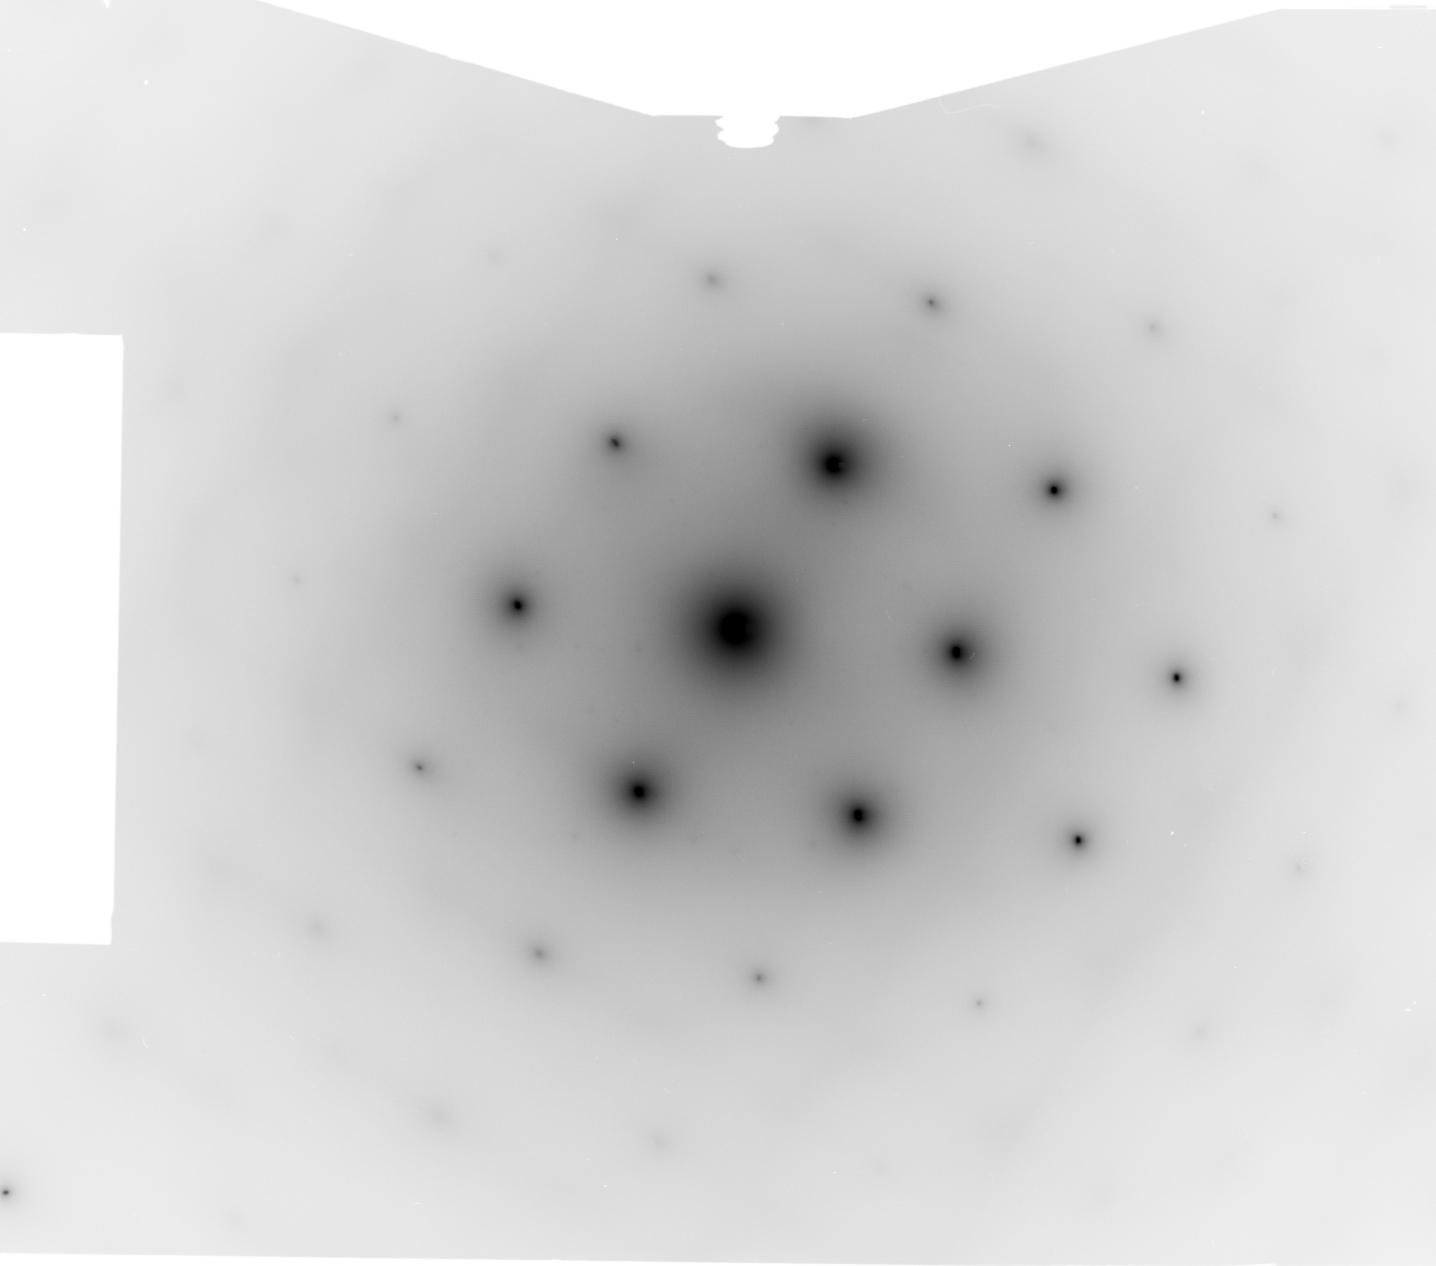
\includegraphics[width=0.45\linewidth]{./Si_Olar.jpg}
\caption{ Si egykristáky diffrakciós képe }
\end{figure}

\end{document}